% Báo cáo Cấp độ 1 — Nhiệm vụ 1 và 2 (Project 3: Truy vấn đa phương thức có giải thích bằng đồ thị)
% Biên dịch bằng XeLaTeX (Overleaf: Menu → Compiler → XeLaTeX).
\documentclass[11pt,a4paper]{article}

\usepackage{fontspec}
\setmainfont{TeX Gyre Termes}
\usepackage[a4paper,margin=2.2cm]{geometry}
\usepackage{amsmath,amssymb}
\usepackage{booktabs,tabularx,multirow,makecell,array,longtable}
\usepackage{xcolor}
\usepackage{graphicx}
\usepackage{caption}
\usepackage{float}
\usepackage{enumitem}
\usepackage{tikz}
\usetikzlibrary{arrows.meta,positioning,fit,backgrounds}
\usepackage{pgfplots}
\pgfplotsset{compat=1.17}
\usepackage[most]{tcolorbox}
\usepackage[hidelinks]{hyperref}

\definecolor{accent}{HTML}{1F5FAD}
\definecolor{good}{HTML}{1E7B34}
\definecolor{bad}{HTML}{B3261E}
\definecolor{soft}{HTML}{EEF3FA}

\captionsetup{font=small,labelfont=bf,labelsep=period}
\captionsetup[table]{name=Bảng}
\captionsetup[figure]{name=Hình}
\renewcommand{\contentsname}{Mục lục}
\renewcommand{\refname}{Tài liệu tham khảo}
\setlist{itemsep=2pt,topsep=4pt}
\newcolumntype{Y}{>{\raggedright\arraybackslash}X}
\newcommand{\clip}{\textsc{clip}}
\newcommand{\pos}[1]{\textcolor{good}{#1}}
\newcommand{\negv}[1]{\textcolor{bad}{#1}}

\title{\textbf{Cấp độ 1 — Nhiệm vụ 1 và 2}\\[4pt]
\large Xếp hạng lại kết quả truy vấn văn bản → ảnh/video bằng CLIP đóng băng và GraphSAGE trên đồ thị dựng từ nhãn có sẵn}
\author{Project 3 — Học máy với dữ liệu đồ thị}
\date{}

\begin{document}
\maketitle

\begin{tcolorbox}[colback=soft,colframe=accent,title=\textbf{Tóm tắt},fonttitle=\small,fontupper=\small]
\begin{itemize}[leftmargin=12pt]
  \item \textbf{Dữ liệu:} hai tập công khai, \textbf{Flickr8k} (văn bản → ảnh) và \textbf{Action Genome} (văn bản → video, mô tả Charades). Dùng split cố định cho mọi cấu hình.
  \item \textbf{Baseline:} OpenCLIP ViT-L/14 (\texttt{laion2b\_s32b\_b82k}), đóng băng, xếp hạng theo cosine.
  \item \textbf{Đồ thị:} đồ thị dị thể ảnh/video – đối tượng – khái niệm – bộ ba, dựng hoàn toàn từ nhãn có sẵn: caption người viết của Flickr8k; nhãn đối tượng, quan hệ của Action Genome và nhãn hành động Charades. Cạnh thống kê chỉ đếm trên tập train.
  \item \textbf{Mô hình:} GraphSAGE 2 lớp có kiểu cạnh, huấn luyện InfoNCE, cộng điểm đường đi trên đồ thị. Xếp hạng lại top-100 của CLIP bằng
  \(s=\alpha\,z(s_{\text{CLIP}})+(1-\alpha)\,[\lambda\,z(s_{\text{GNN}})+(1-\lambda)\,z(s_{\text{path}})]\), với \(\alpha,\lambda\) chọn trên val.
  \item \textbf{Kết quả test} (3 seed): MRR Flickr8k \(0{,}800 \to \mathbf{0{,}832}\) (+0,032, CI 95\% [+0,020; +0,045]); Action Genome \(0{,}171 \to \mathbf{0{,}424}\) (+0,253, CI [+0,236; +0,270]).
  \item \textbf{Ablation:}
  \begin{itemize}[leftmargin=12pt]
    \item Xáo ngẫu nhiên node giữa các ảnh (Flickr8k) làm mất toàn bộ mức tăng: 0,799, ngang CLIP.
    \item Xáo nhãn hành động giữa các video (Action Genome) hạ MRR còn 0,342.
    \item Bỏ cạnh quan hệ hoặc cạnh mức lớp chỉ giảm 0,002–0,008; các khoảng tin cậy đã tính đều chứa 0.
  \end{itemize}
  Mức tăng đến từ \emph{nội dung đúng của liên kết ảnh–node}; cạnh quan hệ giữa các khái niệm đóng góp nhỏ.
  \item \textbf{Giải thích:} mỗi kết quả kèm các đường đi trong đồ thị. Các đường đi này là số hạng của điểm xếp hạng, có phân tích 5 truy vấn thành công và 5 truy vấn thất bại.
\end{itemize}
\end{tcolorbox}

\tableofcontents
\bigskip

%=====================================================================
\section{Yêu cầu của cấp độ 1 và cách đáp ứng}

\begin{table}[H]
\centering\small
\begin{tabularx}{\linewidth}{>{\raggedright\arraybackslash}p{5.2cm}Y}
\toprule
\textbf{Yêu cầu của đề bài} & \textbf{Cách thực hiện (mục)} \\
\midrule
Baseline CLIP đóng băng trên ≥ 1 tập công khai & OpenCLIP ViT-L/14 đóng băng trên Flickr8k và Action Genome (§\ref{sec:baseline}) \\
Dựng đồ thị từ dữ liệu có sẵn (scene graph / nhãn) & Đồ thị ảnh–đối tượng–khái niệm–bộ ba từ caption người viết, nhãn Action Genome, nhãn Charades, WordNet (§\ref{sec:graph}) \\
Ít nhất 1 thuật toán đã học (GCN/GAT/GraphSAGE) & GraphSAGE 2 lớp có kiểu cạnh và cổng, huấn luyện InfoNCE (§\ref{sec:gnn}) \\
Xếp hạng lại bằng kết hợp điểm CLIP và điểm đồ thị & Xếp hạng lại top-100 bằng \(\alpha\,z(\text{CLIP})+(1-\alpha)\,z(\text{đồ thị})\), \(\alpha,\lambda\) chọn trên val (§\ref{sec:rerank}) \\
So sánh CLIP với CLIP + Graph trên cùng cách chia & Cùng split, cùng tập ứng viên, 3 seed, bootstrap cặp (§\ref{sec:results}) \\
Ablation: bỏ cạnh hoặc thay bằng cạnh ngẫu nhiên & Bỏ cạnh quan hệ, bỏ cạnh mức lớp, xáo node / nhãn ngẫu nhiên giữa các mẫu (§\ref{sec:ablation}) \\
Hiển thị quan hệ / đường đi khi xếp hạng & 7 mẫu đường đi P0–P6, đóng góp biên của từng đường đi, hàm \texttt{demo\_query()} (§\ref{sec:explain}) \\
Phân tích 5 truy vấn thành công và 5 truy vấn thất bại & Chọn theo luật cố định trên test, trên cả hai tập (§\ref{sec:cases}) \\
\bottomrule
\end{tabularx}
\caption{Đối chiếu yêu cầu cấp độ 1 với phần đã làm.}
\end{table}

%=====================================================================
\section{Dữ liệu và cách chia}\label{sec:data}

\begin{table}[H]
\centering\small
\begin{tabular}{lcc}
\toprule
 & \textbf{Flickr8k} & \textbf{Action Genome} \\
\midrule
Chiều truy vấn & văn bản → ảnh & văn bản → video \\
Số mẫu gallery & 8.000 ảnh & 9.587 video \\
Split (train / val / test) & 6.000 / 1.000 / 1.000 & 6.611 / 1.166 / 1.810 \\
Nguồn split & split chính thức (HF) & train/test gốc của AG; val tách từ train bằng seed cố định \\
Truy vấn & caption số 0 của mỗi ảnh & mô tả Charades của video \\
Số truy vấn test & 1.000 & 1.810 \\
Đáp án & 1 ảnh & 1 video \\
\bottomrule
\end{tabular}
\caption{Hai tập công khai. Mỗi truy vấn có đúng một đáp án; gallery của mỗi phần là toàn bộ ảnh/video của phần đó.}
\label{tab:data}
\end{table}

\paragraph{Chống rò rỉ dữ liệu.}
\begin{itemize}
  \item Split cố định, kiểm tra bằng mã băm (Flickr8k \texttt{sha1=005202c6\ldots}, AG \texttt{sha1=1f1f4e81\ldots}); mọi cấu hình và seed dùng cùng split.
  \item Từ vựng đối tượng, cạnh \emph{scene}, cạnh \emph{related}, IDF và trọng số cạnh chỉ đếm trên \textbf{train}. Self-test trong notebook kiểm tra điều này.
  \item GNN chỉ huấn luyện trên truy vấn train.
  \item \(\alpha\) và \(\lambda\) chỉ chọn trên \textbf{val}; tập test chỉ dùng để báo cáo.
\end{itemize}

\paragraph{Lưu ý về nguồn node của Flickr8k.} Node của mỗi ảnh Flickr8k lấy từ \emph{caption 1–4 do người viết}, còn truy vấn là caption 0 của cùng ảnh. Đây là kịch bản \emph{gallery đã được chú thích} (giống ảnh có tag hoặc mô tả sẵn). Caption 0 không bao giờ được dùng làm node.

Ở các phiên bản trước, node sinh tự động từ ảnh (CLIP tagger, linear probe, BLIP caption). Với cách đó đồ thị chỉ tăng tối đa +0,007 MRR. Vì vậy, kết luận của báo cáo này chỉ áp dụng khi gallery có nhãn của con người.

%=====================================================================
\section{Baseline CLIP đóng băng}\label{sec:baseline}

\begin{itemize}
  \item \textbf{Mô hình:} OpenCLIP \texttt{ViT-L-14}, trọng số \texttt{laion2b\_s32b\_b82k}. Không tinh chỉnh.
  \item \textbf{Đặc trưng:} trích một lần cho mọi ảnh, video và truy vấn rồi lưu cache. Mỗi video Action Genome lấy 4 frame; đặc trưng video là trung bình đặc trưng các frame, chuẩn hoá L2.
  \item \textbf{Điểm:} \(s_{\text{CLIP}}(q,v)=\cos\big(f_T(q), f_I(v)\big)\), xếp hạng toàn bộ gallery test.
  \item \textbf{Ứng viên cho xếp hạng lại:} top-\(K\) với \(K=100\) theo \(s_{\text{CLIP}}\). Ảnh/video ngoài top-100 giữ nguyên thứ tự CLIP, nên CLIP và CLIP + Graph có cùng trần R@100.
\end{itemize}

%=====================================================================
\section{Dựng đồ thị từ dữ liệu có sẵn}\label{sec:graph}

\subsection{Đỉnh và cạnh}
Đồ thị là đồ thị dị thể tĩnh \(G=(V,E)\). Hình~\ref{fig:schema} minh hoạ lược đồ.
\begin{itemize}
  \item \textbf{Đỉnh ảnh/video} \(v\): mỗi mẫu trong gallery (cả train, val, test).
  \item \textbf{Đỉnh đối tượng / cụm từ} \(o\):
  \begin{itemize}
    \item Flickr8k: danh từ và cụm 2 từ rút từ caption 1–4, giữ lớp xuất hiện ≥ 5 lần trên train.
    \item Action Genome: lớp đối tượng của AG, node hành động Charades (vd \textit{open door}, \textit{look television}) và node bối cảnh (vd \textit{bedroom}).
  \end{itemize}
  \item \textbf{Đỉnh khái niệm} \(c\): hypernym WordNet của lớp đối tượng, đã lọc khái niệm quá chung (\textit{entity, object\ldots}).
  \item \textbf{Đỉnh bộ ba} \(t\):
  \begin{itemize}
    \item Flickr8k: \(\langle\)chủ thể, vị từ, đối tượng\(\rangle\) rút từ caption người viết.
    \item Action Genome: bộ ba thời gian \(\langle a \text{ trước } b\rangle\) từ chuỗi hành động Charades.
  \end{itemize}
\end{itemize}

Có 5 loại cạnh:
\begin{enumerate}
  \item \texttt{chứa} (ảnh → đối tượng): nhãn riêng của từng mẫu.
  \item \texttt{scene} (đối tượng → đối tượng): quan hệ trong scene graph hoặc caption, xuất hiện ≥ 2 lần trên train, tối đa 10 cạnh mạnh nhất mỗi lớp.
  \item \texttt{liên\_quan} (đối tượng → đối tượng): đồng xuất hiện trên train, xếp hạng theo NPMI (≥ 0,10), tối đa 10 cạnh mỗi lớp, trọng số \(P(\text{đích}\mid\text{nguồn})\).
  \item \texttt{là\_một} (đối tượng → khái niệm): quan hệ IsA của WordNet.
  \item \texttt{thể\_hiện} (ảnh → bộ ba).
\end{enumerate}
Các cạnh \texttt{scene}, \texttt{liên\_quan} và \texttt{là\_một} gọi chung là \emph{cạnh mức lớp}.

\begin{figure}[H]
\centering
\begin{tikzpicture}[
  node distance=1.3cm and 1.9cm,
  every node/.style={font=\small},
  img/.style={draw=accent,fill=soft,rounded corners=2pt,minimum width=1.7cm,minimum height=0.7cm},
  obj/.style={draw=good,fill=good!8,rounded corners=8pt,minimum height=0.6cm},
  con/.style={draw=orange!80!black,fill=orange!10,rounded corners=8pt,minimum height=0.6cm},
  tri/.style={draw=purple!70!black,fill=purple!8,minimum height=0.6cm},
  e/.style={-{Stealth[length=2.2mm]},thick}]
\node[img] (v) {ảnh \(v\)};
\node[obj, right=of v, yshift=1.0cm] (o1) {snowboarder};
\node[obj, right=of v, yshift=-0.2cm] (o2) {grinding};
\node[tri, below=0.8cm of v] (t) {\(\langle\)man, ride, snowboard\(\rangle\)};
\node[obj, right=2.1cm of o1] (o3) {snowboard};
\node[con, right=2.1cm of o2] (c1) {person};
\draw[e] (v) -- node[above,sloped,font=\scriptsize]{chứa} (o1);
\draw[e] (v) -- node[below,sloped,font=\scriptsize]{chứa} (o2);
\draw[e] (v) -- node[left,font=\scriptsize]{thể\_hiện} (t);
\draw[e] (o1) -- node[above,font=\scriptsize]{liên\_quan} (o3);
\draw[e] (o1) -- node[above,sloped,font=\scriptsize,pos=0.4]{là\_một} (c1);
\node[draw=gray,dashed,rounded corners,fit=(o3)(c1),inner sep=6pt,label={[font=\scriptsize,gray]below:khái niệm trong truy vấn}] {};
\end{tikzpicture}
\caption{Lược đồ đồ thị. Đường đi từ ảnh tới khái niệm xuất hiện trong truy vấn (vd \textit{snowboard}) là bằng chứng để xếp hạng và để giải thích.}
\label{fig:schema}
\end{figure}

\subsection{Thống kê đồ thị}
\begin{table}[H]
\centering\small
\begin{tabular}{lrr}
\toprule
 & \textbf{Flickr8k} & \textbf{Action Genome} \\
\midrule
Tổng số đỉnh & 35.104 & 28.494 \\
\quad đỉnh ảnh / video & 8.000 & 9.587 \\
\quad đỉnh đối tượng / cụm từ / hành động & 5.353 & 333 \\
\quad đỉnh khái niệm WordNet & 509 & 88 \\
\quad đỉnh bộ ba & 21.242 & 18.486 \\
Cạnh \texttt{chứa} & 200.335 & 162.491 \\
Cạnh \texttt{scene} / \texttt{liên\_quan} / \texttt{là\_một} & 1.503 / 11.699 / 1.930 & 266 / 2.987 / 353 \\
Cạnh \texttt{thể\_hiện} (ảnh → bộ ba) & 33.459 & 193.428 \\
Số node trung bình mỗi mẫu & 37,0 & 17,0 (+ 11,3 hành động/bối cảnh) \\
\bottomrule
\end{tabular}
\caption{Thống kê đồ thị đầy đủ (cấu hình \texttt{none}), lấy từ log lần chạy Kaggle.}
\label{tab:graphstats}
\end{table}

%=====================================================================
\section{Thuật toán đồ thị đã học: GraphSAGE}\label{sec:gnn}

\paragraph{Biểu diễn đỉnh.}
\begin{itemize}
  \item Đỉnh ảnh/video: \(h^{(0)}_v=W_{\text{img}}f_I(v)\), tức chiếu từ đặc trưng CLIP đóng băng. Vì vậy mô hình là \emph{inductive}: ảnh test chưa từng dùng khi huấn luyện vẫn có biểu diễn hợp lệ.
  \item Đỉnh đối tượng, khái niệm, bộ ba: embedding học được, vì các đỉnh này lặp lại giữa nhiều ảnh.
\end{itemize}

\paragraph{Lớp GraphSAGE có kiểu cạnh.} Mỗi loại cạnh \(t\), xét theo cả hai chiều, có ma trận riêng và một cổng học được:
\[
h^{(l+1)}_v=\mathrm{LN}\Big(W_0h^{(l)}_v+\sum_{t}\sigma(g_t)\,W_t\,\underset{u\in\mathcal N_t(v)}{\mathrm{mean}}\,h^{(l)}_u\Big).
\]
Cổng của cạnh \texttt{chứa} khởi tạo mở. Cổng của các cạnh mức lớp khởi tạo gần đóng (\(\sigma(-1{,}5)\approx 0{,}18\)): mô hình bắt đầu gần cấu hình "không quan hệ", và chỉ mở thêm quan hệ khi việc đó giảm loss. Cấu hình: 2 lớp, 256 chiều, dropout 0,1, GELU giữa hai lớp, chuẩn hoá L2 ở đầu ra.

\paragraph{Điểm GNN.} Truy vấn được chiếu từ CLIP-text sang không gian đồ thị bằng MLP 2 lớp:
\[
s_{\text{GNN}}(q,v)=\cos\big(\mathrm{MLP}(f_T(q)),\,h^{(L)}_v\big).
\]

\paragraph{Điểm đường đi.} Các khái niệm trong truy vấn được nhận ra bằng khớp n-gram (1–2 từ, bỏ stop-word) với tên đỉnh. Với mỗi ứng viên \(v\), liệt kê đường đi từ \(v\) tới các khái niệm đó theo 7 mẫu (Bảng~\ref{tab:patterns}).
\begin{itemize}
  \item Trọng số của một đường đi = IDF của đỉnh đích × tích trọng số các cạnh trên đường đi.
  \item Tổng theo mẫu được nén bằng \(\log(1+\cdot)\).
  \item \(s_{\text{path}}(q,v)=\sum_p w_p\log\big(1+\sum_{\pi\in p}w_\pi\big)\), với \(w_{P0}=1\) và \(w_p=\mathrm{softplus}(\theta_p)\,\delta^{|p|-1}\) học được, \(\delta\) là hệ số suy giảm theo độ dài.
\end{itemize}

\paragraph{Huấn luyện.}
\begin{itemize}
  \item Loss InfoNCE trên truy vấn train, gồm hai số hạng: âm trong batch, và 31 ảnh âm khó lấy từ top-\(K\) CLIP trên gallery train.
  \item Logit huấn luyện gồm \(z(s_{\text{GNN}})\), \(z(s_{\text{path}})\) và \(z(s_{\text{CLIP}})\). Nhờ có \(z(s_{\text{CLIP}})\), đồ thị học phần CLIP còn thiếu thay vì học lại CLIP. Hệ số của \(z(s_{\text{CLIP}})\) học được hay cố định được chọn trên val.
  \item Siêu tham số: AdamW, lr \(10^{-3}\), weight decay \(10^{-4}\), 20 epoch, batch 128, nhiệt độ 0,07.
  \item CLIP luôn đóng băng.
\end{itemize}

%=====================================================================
\section{Xếp hạng lại bằng kết hợp điểm}\label{sec:rerank}

Với mỗi truy vấn, chuẩn hoá z từng điểm trên tập top-100 ứng viên rồi trộn:
\[
\boxed{\;s(q,v)=\alpha\,z\big(s_{\text{CLIP}}\big)+(1-\alpha)\Big[\lambda\,z\big(s_{\text{GNN}}\big)+(1-\lambda)\,z\big(s_{\text{path}}\big)\Big]\;}
\]
\begin{itemize}
  \item Chuẩn hoá z cho ba điểm cùng thang đo, nên \(\alpha\) chọn trên val dùng được cho test.
  \item Lưới: \(\alpha\in\{0;0{,}2;0{,}4;0{,}5;0{,}6;0{,}7;0{,}8;0{,}9;1\}\), \(\lambda\in\{0;0{,}25;0{,}5;0{,}75\}\). Bỏ \(\lambda=1\) vì khi đó \(s_{\text{path}}\) có trọng số 0 và đường đi giải thích không còn ảnh hưởng tới điểm.
  \item Chọn theo MRR trên val, riêng cho từng seed. \(\alpha=1\) chính là CLIP thuần.
  \item Giá trị được chọn: Flickr8k \(\alpha\in\{0{,}5;0{,}6\}\), \(\lambda=0{,}25\). Action Genome \(\alpha\in\{0;0{,}2\}\), \(\lambda\in\{0{,}25;0{,}5\}\): CLIP rất yếu trên AG nên val chọn dựa gần như hoàn toàn vào đồ thị, CLIP chỉ còn dùng để lấy ứng viên.
\end{itemize}

\begin{figure}[H]
\centering
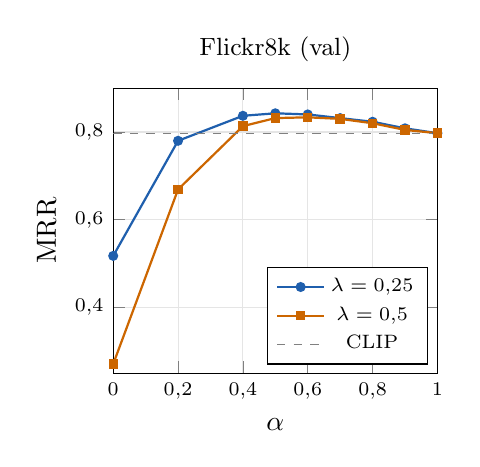
\begin{tikzpicture}
\begin{axis}[
  width=0.47\linewidth, height=5.2cm,
  title={\small Flickr8k (val)}, xlabel={\(\alpha\)}, ylabel={MRR},
  xmin=0,xmax=1, ymin=0.25,ymax=0.9, grid=major, grid style={gray!20},
  legend style={font=\scriptsize,at={(0.97,0.03)},anchor=south east},
  tick label style={font=\scriptsize},
  /pgf/number format/use comma]
\addplot[accent,thick,mark=*,mark size=1.4pt] coordinates {(0,0.5174)(0.2,0.7800)(0.4,0.8370)(0.5,0.8427)(0.6,0.8401)(0.7,0.8317)(0.8,0.8234)(0.9,0.8084)(1,0.7973)};
\addplot[orange!80!black,thick,mark=square*,mark size=1.3pt] coordinates {(0,0.2707)(0.2,0.6690)(0.4,0.8134)(0.5,0.8318)(0.6,0.8335)(0.7,0.8300)(0.8,0.8200)(0.9,0.8048)(1,0.7973)};
\addplot[gray,dashed] coordinates {(0,0.7973)(1,0.7973)};
\legend{\(\lambda=0{,}25\),\(\lambda=0{,}5\),CLIP}
\end{axis}
\end{tikzpicture}\hfill
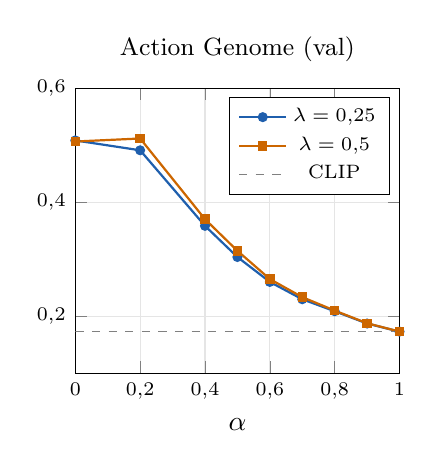
\begin{tikzpicture}
\begin{axis}[
  width=0.47\linewidth, height=5.2cm,
  title={\small Action Genome (val)}, xlabel={\(\alpha\)},
  xmin=0,xmax=1, ymin=0.1,ymax=0.6, grid=major, grid style={gray!20},
  legend style={font=\scriptsize,at={(0.97,0.97)},anchor=north east},
  tick label style={font=\scriptsize},
  /pgf/number format/use comma]
\addplot[accent,thick,mark=*,mark size=1.4pt] coordinates {(0,0.5083)(0.2,0.4910)(0.4,0.3584)(0.5,0.3037)(0.6,0.2600)(0.7,0.2296)(0.8,0.2086)(0.9,0.1870)(1,0.1728)};
\addplot[orange!80!black,thick,mark=square*,mark size=1.3pt] coordinates {(0,0.5064)(0.2,0.5117)(0.4,0.3701)(0.5,0.3146)(0.6,0.2650)(0.7,0.2333)(0.8,0.2097)(0.9,0.1875)(1,0.1728)};
\addplot[gray,dashed] coordinates {(0,0.1728)(1,0.1728)};
\legend{\(\lambda=0{,}25\),\(\lambda=0{,}5\),CLIP}
\end{axis}
\end{tikzpicture}
\caption{MRR trên \textbf{val} theo \(\alpha\) (seed 0). \(\alpha=1\) là CLIP thuần.
Flickr8k: tốt nhất ở \(\alpha\approx 0{,}5\); bỏ hẳn CLIP (\(\alpha=0\)) làm kết quả tệ đi.
Action Genome: MRR tăng đều khi giảm \(\alpha\), vì đồ thị mang thông tin hành động mà CLIP không thấy.}
\label{fig:alpha}
\end{figure}

%=====================================================================
\section{Kết quả: CLIP và CLIP + Graph trên cùng cách chia}\label{sec:results}

\paragraph{Thiết lập so sánh.} Hai mô hình dùng cùng split, cùng truy vấn test và cùng top-100 ứng viên. CLIP là tất định nên độ lệch chuẩn bằng 0. CLIP + Graph chạy 3 seed huấn luyện (0, 1, 2), báo cáo trung bình ± độ lệch chuẩn. Khoảng tin cậy 95\% tính bằng bootstrap cặp theo truy vấn, 10.000 lần, trên RR đã lấy trung bình theo seed.

\begin{table}[H]
\centering\small
\setlength{\tabcolsep}{5pt}
\begin{tabular}{llccccc}
\toprule
\textbf{Tập} & \textbf{Mô hình} & \textbf{R@1} & \textbf{R@5} & \textbf{R@10} & \textbf{MRR} & \textbf{nDCG@10} \\
\midrule
\multirow{3}{*}{\makecell[l]{Flickr8k\\ (1.000 truy vấn)}}
 & CLIP & 0,706 & 0,913 & 0,969 & 0,800 & 0,839 \\
 & CLIP + Graph & \textbf{0,750} \scriptsize{±0,004} & \textbf{0,939} \scriptsize{±0,001} & \textbf{0,973} \scriptsize{±0,001} & \textbf{0,832} \scriptsize{±0,003} & \textbf{0,865} \scriptsize{±0,002} \\
 & \(\Delta\) & \pos{+0,044} & \pos{+0,026} & \pos{+0,004} & \pos{+0,032} & \pos{+0,026} \\
\midrule
\multirow{3}{*}{\makecell[l]{Action Genome\\ (1.810 truy vấn)}}
 & CLIP & 0,104 & 0,234 & 0,313 & 0,171 & 0,195 \\
 & CLIP + Graph & \textbf{0,335} \scriptsize{±0,009} & \textbf{0,536} \scriptsize{±0,010} & \textbf{0,595} \scriptsize{±0,012} & \textbf{0,424} \scriptsize{±0,008} & \textbf{0,463} \scriptsize{±0,010} \\
 & \(\Delta\) & \pos{+0,231} & \pos{+0,301} & \pos{+0,282} & \pos{+0,253} & \pos{+0,267} \\
\bottomrule
\end{tabular}
\caption{Kết quả trên \textbf{test}. CLIP + Graph = GraphSAGE + điểm đường đi, xếp hạng lại top-100 của CLIP. R@1 chính là độ chính xác top-1.}
\label{tab:main}
\end{table}

\begin{table}[H]
\centering\small
\begin{tabular}{lcc}
\toprule
\textbf{Tập} & \(\Delta\)\textbf{MRR} (CLIP + Graph − CLIP) & \textbf{CI 95\%} \\
\midrule
Flickr8k & \pos{+0,032} & [+0,020; +0,045] \\
Action Genome & \pos{+0,253} & [+0,236; +0,270] \\
\bottomrule
\end{tabular}
\caption{Kiểm định bootstrap cặp theo truy vấn (10.000 lần). Cả hai mức tăng đều có ý nghĩa: khoảng tin cậy không chứa 0.}
\label{tab:paired}
\end{table}

\paragraph{Nhận xét.}
\begin{itemize}
  \item \textbf{Action Genome}, mức tăng lớn (MRR ×2,5; R@1 từ 10\% lên 34\%).
  \begin{itemize}
    \item CLIP rất yếu trên video Charades: quay trong nhà, tối, các video rất giống nhau, mỗi video chỉ biểu diễn bằng 4 frame gộp lại.
    \item Đồ thị mang thông tin CLIP không thấy được từ ảnh, như hành động (\textit{look television}), bối cảnh phòng và thứ tự hành động.
  \end{itemize}
  \item \textbf{Flickr8k}, mức tăng nhỏ nhưng có ý nghĩa (+0,032 MRR, +4,4 điểm R@1). CLIP đã mạnh (R@10 = 96,9\%), nên đồ thị chủ yếu sửa thứ hạng trong top-10.
  \item R@10 Flickr8k gần như không đổi (+0,004): khi đáp án đã nằm trong top-10 của CLIP, đồ thị chỉ đẩy nó lên cao hơn.
\end{itemize}

%=====================================================================
\section{Ablation: bỏ cạnh và thay bằng liên kết ngẫu nhiên}\label{sec:ablation}

Mỗi cấu hình ablation dựng lại đồ thị, huấn luyện lại GNN với 3 seed và chọn lại \(\alpha,\lambda\) trên val, đúng quy trình của mô hình đầy đủ:
\begin{itemize}
  \item \texttt{no\_class\_edges}: bỏ toàn bộ cạnh mức lớp (\texttt{scene}, \texttt{liên\_quan}, \texttt{là\_một}); chỉ còn cạnh \texttt{chứa} và \texttt{thể\_hiện}.
  \item \texttt{no\_relations}: bỏ thêm đỉnh khái niệm và đỉnh bộ ba; chỉ còn cạnh \texttt{chứa}.
  \item \texttt{shuffled\_nodes} (Flickr8k): hoán vị ngẫu nhiên tập node giữa các ảnh. Bậc của mỗi ảnh và phân phối node giữ nguyên, nhưng liên kết ảnh–node thành ngẫu nhiên. Đây là phép "thay bằng cạnh ngẫu nhiên".
  \item \texttt{shuffled\_actions} (Action Genome): hoán vị nhãn hành động/bối cảnh giữa các video.
  \item \texttt{no\_actions} (Action Genome): bỏ node hành động/bối cảnh Charades.
\end{itemize}

\begin{table}[H]
\centering\small
\begin{tabular}{llccc}
\toprule
\textbf{Tập} & \textbf{Cấu hình} & \textbf{R@1} & \textbf{MRR} & \textbf{Đầy đủ hơn cấu hình này (CI 95\%)} \\
\midrule
\multirow{5}{*}{Flickr8k}
 & CLIP & 0,706 & 0,800 & +0,032 [+0,020; +0,045] \\
 & \textbf{CLIP + Graph (đầy đủ)} & \textbf{0,750} & \textbf{0,832} & — \\
 & bỏ cạnh mức lớp & 0,745 & 0,828 & +0,004 (không có kiểm định cặp) \\
 & bỏ quan hệ (chỉ còn \texttt{chứa}) & 0,747 & 0,830 & +0,002 [−0,004; +0,008] \\
 & \negv{node xáo ngẫu nhiên} & 0,707 & \negv{0,799} & +0,034 [+0,021; +0,046] \\
\midrule
\multirow{6}{*}{Action Genome}
 & CLIP & 0,104 & 0,171 & +0,253 [+0,236; +0,270] \\
 & \textbf{CLIP + Graph (đầy đủ)} & \textbf{0,335} & \textbf{0,424} & — \\
 & bỏ cạnh mức lớp & 0,329 & 0,418 & +0,006 [−0,001; +0,012] \\
 & bỏ quan hệ & 0,329 & 0,416 & +0,008 [−0,003; +0,019] \\
 & bỏ node hành động & 0,280 & 0,377 & +0,048 [+0,037; +0,058] \\
 & \negv{nhãn hành động xáo ngẫu nhiên} & 0,243 & \negv{0,342} & +0,083 [+0,071; +0,094] \\
\bottomrule
\end{tabular}
\caption{Ablation trên \textbf{test} (trung bình 3 seed). Cột cuối: hiệu MRR giữa mô hình đầy đủ và cấu hình đó, bootstrap cặp. Dòng "bỏ cạnh mức lớp" của Flickr8k không có file kiểm định cặp nên chỉ ghi hiệu trung bình.}
\label{tab:ablation}
\end{table}

\paragraph{Kết luận ablation.}
\begin{enumerate}
  \item \textbf{Thay liên kết bằng liên kết ngẫu nhiên làm mất mức tăng.}
  \begin{itemize}
    \item Flickr8k: xáo node đưa MRR về 0,799, ngang CLIP (0,800).
    \item Action Genome: xáo nhãn hành động làm MRR giảm 0,083 so với mô hình đầy đủ, xuống dưới cả cấu hình bỏ hẳn node hành động (0,342 so với 0,377). Nhãn sai còn gây hại hơn không có nhãn.
  \end{itemize}
  Mức tăng vì vậy đến từ \emph{nội dung đúng} của đồ thị, không đến từ việc thêm tham số hay thêm một nhánh điểm.
  \item \textbf{Cạnh quan hệ giữa các khái niệm đóng góp nhỏ.} Bỏ \texttt{scene}/\texttt{liên\_quan}/\texttt{là\_một}, hoặc bỏ cả đỉnh khái niệm và bộ ba, chỉ giảm 0,002–0,008 MRR; các khoảng tin cậy đã tính đều chứa 0. Phần lớn mức tăng đi qua cạnh \texttt{chứa} (liên kết ảnh–nhãn) và qua GraphSAGE lan truyền trên các cạnh đó.
  \item Với cấp độ 1, kết luận cần nói đúng như sau: \emph{cấu trúc liên kết ảnh–nhãn đúng} là nguồn cải thiện. Các cạnh quan hệ mức lớp mới chỉ cho tác dụng nhỏ, chưa chứng minh được rõ.
\end{enumerate}

\paragraph{Kết quả âm trên scene graph Visual Genome.}
Phần B của dự án chạy pipeline tương tự trên \textbf{Visual Genome + COCO} với scene graph gốc của VG (3 seed; Bảng~\ref{tab:vg}). Trên tập này GraphSAGE \emph{không} hơn CLIP, và đồ thị ngẫu nhiên hay bỏ cạnh cho kết quả gần như nhau. Kết quả này nhất quán với Flickr8k: khi CLIP đã mạnh và đồ thị chỉ mô tả lại các vật thể mà CLIP đã thấy trong ảnh, đồ thị gần như không thêm thông tin.

\begin{table}[H]
\centering\small
\begin{tabular}{lcc}
\toprule
\textbf{Cấu hình (VG + COCO, văn bản → ảnh)} & \textbf{R@1 (\%)} & \textbf{MRR} \\
\midrule
CLIP & 61,1 & 0,718 \\
GraphSAGE (ảnh – lớp – bộ ba) & 61,1 & 0,718 \\
GraphSAGE, cạnh ngẫu nhiên & 61,1 & 0,718 \\
GraphSAGE, bỏ cạnh & 60,9 & 0,717 \\
\bottomrule
\end{tabular}
\caption{GraphSAGE trên scene graph Visual Genome (phần B, \texttt{results/partB\_image\_video/}). Không cấu hình đồ thị nào hơn CLIP.}
\label{tab:vg}
\end{table}

%=====================================================================
\section{Giải thích: quan hệ và đường đi dùng khi xếp hạng}\label{sec:explain}

\paragraph{Giải thích đến từ chính cơ chế xếp hạng.} Giải thích là các đường đi nằm trong số hạng \(s_{\text{path}}\) của điểm cuối, với trọng số \((1-\alpha)(1-\lambda)>0\). Điểm cuối thay đổi khi các đường đi đó bị xoá; giải thích không phải đường đi hợp lý được ghép thêm sau khi đã xếp hạng.

\paragraph{Cách tính đóng góp.} Đóng góp của một đường đi \(\pi\) là \emph{đóng góp biên}: \(s_{\text{path}}(\text{mọi đường}) - s_{\text{path}}(\text{mọi đường} \setminus \{\pi\})\). Giải thích hiển thị tối đa 5 đường đi có đóng góp lớn nhất. Notebook có self-test kiểm tra rằng tổng theo mẫu của các đường đi liệt kê khớp tuyệt đối với điểm tính bằng ma trận (299/299 cặp).

\begin{table}[H]
\centering\small
\begin{tabular}{llc}
\toprule
\textbf{Mẫu} & \textbf{Dạng đường đi} & \textbf{Độ dài} \\
\midrule
P0 & ảnh \(\xrightarrow{\text{chứa}}\) \(c\) & 1 \\
P1 & ảnh \(\xrightarrow{\text{chứa}}\) \(o\) \(\xrightarrow{\text{scene}}\) \(c\) & 2 \\
P2 & ảnh \(\xrightarrow{\text{chứa}}\) \(o\) \(\xrightarrow{\text{là\_một}}\) \(c\) & 2 \\
P3 & ảnh \(\xrightarrow{\text{chứa}}\) \(o\) \(\xrightarrow{\text{liên\_quan}}\) \(c\) & 2 \\
P4 & ảnh \(\xrightarrow{\text{chứa}}\) \(o\) \(\xrightarrow{\text{scene}}\) \(o'\) \(\xrightarrow{\text{là\_một}}\) \(c\) & 3 \\
P5 & ảnh \(\xrightarrow{\text{chứa}}\) \(o\) \(\xrightarrow{\text{liên\_quan}}\) \(o'\) \(\xrightarrow{\text{là\_một}}\) \(c\) & 3 \\
P6 & ảnh \(\xrightarrow{\text{thể\_hiện}}\) \(\langle s,p,o\rangle\) & 1 \\
\bottomrule
\end{tabular}
\caption{Bảy mẫu đường đi từ ứng viên tới khái niệm \(c\) trong truy vấn.}
\label{tab:patterns}
\end{table}

\paragraph{Ví dụ đầu ra của \texttt{demo\_query()}.} Truy vấn Flickr8k \textit{"A guy on a snowboard grinding."}: CLIP xếp ảnh đúng ở hạng 14, CLIP + Graph đưa lên hạng 4, với giải thích:
\begin{quote}\small
ảnh \(\xrightarrow{\text{chứa}}\) grinding \hfill [P0, đóng góp +2,48]\\
ảnh \(\xrightarrow{\text{chứa}}\) snowboarder \(\xrightarrow{\text{liên\_quan}}\) snowboard \hfill [P3, +0,28]\\
ảnh \(\xrightarrow{\text{chứa}}\) pant \(\xrightarrow{\text{liên\_quan}}\) snowboard \hfill [P3, +0,03]
\end{quote}
Bỏ 3 đường đi này, điểm đường đi của ảnh từ 2,86 về 0,00. Bỏ ngẫu nhiên 3 đường đi, điểm còn 0,89 (trung bình 10 lần bốc).

\paragraph{Kiểm tra định lượng.} Xét 20 truy vấn test mỗi tập (Bảng~\ref{tab:fid}).
\begin{itemize}
  \item Bỏ đúng các đường đi trong giải thích làm điểm đường đi tụt nhiều hơn hẳn so với bỏ cùng số đường đi ngẫu nhiên: Flickr8k 2,69 so với 1,12; Action Genome 2,40 so với 0,42.
  \item Mọi đường đi trong giải thích đều kết thúc ở một khái niệm có trong truy vấn (validity = 1).
\end{itemize}
Đánh giá đầy đủ fidelity, validity, sparsity thuộc cấp độ 3; ở đây chỉ dùng để xác nhận giải thích bám vào điểm.

\begin{table}[H]
\centering\small
\begin{tabular}{lcc}
\toprule
 & \textbf{Flickr8k} & \textbf{Action Genome} \\
\midrule
Số truy vấn & 20 & 20 \\
Số đường đi trung bình / cặp (truy vấn, ảnh đúng) & 10,5 & 38,1 \\
Điểm tụt khi bỏ đường đi giải thích & \textbf{2,69} & \textbf{2,40} \\
Điểm tụt khi bỏ cùng số đường đi ngẫu nhiên & 1,12 & 0,42 \\
Validity (đường đi tới khái niệm có trong truy vấn) & 1,00 & 1,00 \\
Sparsity (tỉ lệ đường đi \emph{không} nằm trong giải thích) & 0,50 & 0,80 \\
\bottomrule
\end{tabular}
\caption{Giải thích bám vào điểm xếp hạng (\texttt{xai\_summary.json}).}
\label{tab:fid}
\end{table}

%=====================================================================
\section{Phân tích 5 truy vấn thành công và 5 truy vấn thất bại}\label{sec:cases}

\paragraph{Luật chọn ca.} Luật cố định trong hàm \texttt{analyse\_cases}, không chọn tay, áp dụng trên test, seed 0, mô hình CLIP + Graph:
\begin{itemize}
  \item \emph{Thành công:} 5 truy vấn được đồ thị kéo lên nhiều hạng nhất và có đáp án nằm trong top-10 sau xếp hạng lại.
  \item \emph{Thất bại:} 5 truy vấn bị đồ thị đẩy xuống nhiều hạng nhất so với CLIP.
\end{itemize}

\paragraph{Cách đọc các bảng.}
\begin{itemize}
  \item Cột "Hạng": hạng của đáp án đúng, CLIP → CLIP + Graph.
  \item Cột "Đường đi": 3 đường đi đóng góp nhiều nhất cho ảnh đúng, kèm mẫu và đóng góp biên.
  \item Cột "Tụt": điểm đường đi giảm bao nhiêu khi bỏ các đường đi giải thích / khi bỏ cùng số đường đi ngẫu nhiên.
\end{itemize}

\subsection{Flickr8k}

{\small
\renewcommand{\arraystretch}{1.25}
\begin{longtable}{>{\centering\arraybackslash}p{0.3cm}>{\raggedright\arraybackslash}p{3.6cm}>{\centering\arraybackslash}p{1.25cm}>{\centering\arraybackslash}p{1.1cm}>{\raggedright\arraybackslash}p{6.4cm}>{\centering\arraybackslash}p{1.4cm}}
\caption{Flickr8k: 5 thành công (trên) và 5 thất bại (dưới).}\label{tab:cases_f8k}\\
\toprule
\# & \textbf{Truy vấn} & \textbf{Nhóm} & \textbf{Hạng} & \textbf{Đường đi tới ảnh đúng} \footnotesize[mẫu, đóng góp] & \textbf{Tụt} \footnotesize giải thích / ngẫu nhiên \\
\midrule
\endfirsthead
\toprule
\# & \textbf{Truy vấn} & \textbf{Nhóm} & \textbf{Hạng} & \textbf{Đường đi} & \textbf{Tụt} \\
\midrule
\endhead
\multicolumn{6}{l}{\textcolor{good}{\textbf{Thành công}}}\\
1 & \textit{A football player in blue and one in red play in a game .} & trực tiếp & 30\(\to\)9 & ảnh \(\xrightarrow{\text{\scriptsize chứa}}\) football player \hfill{\footnotesize[P0, +0,31]} \newline ảnh \(\xrightarrow{\text{\scriptsize chứa}}\) football \hfill{\footnotesize[P0, +0,27]} \newline ảnh \(\xrightarrow{\text{\scriptsize chứa}}\) game \hfill{\footnotesize[P0, +0,22]} & 2,03 / 1,16 \\
2 & \textit{A lady looks to her right and holds a mini camera .} & trực tiếp & 19\(\to\)8 & ảnh \(\xrightarrow{\text{\scriptsize chứa}}\) lady \hfill{\footnotesize[P0, +0,89]} \newline ảnh \(\xrightarrow{\text{\scriptsize chứa}}\) camera \hfill{\footnotesize[P0, +0,63]} \newline ảnh \(\xrightarrow{\text{\scriptsize chứa}}\) woman holding \(\xrightarrow{\text{\scriptsize liên\_quan}}\) hold \hfill{\footnotesize[P3, +0,15]} & 2,83 / 2,32 \\
3 & \textit{Children play with large hoops .} & trực tiếp & 21\(\to\)10 & ảnh \(\xrightarrow{\text{\scriptsize chứa}}\) play \hfill{\footnotesize[P0, +0,75]} \newline ảnh \(\xrightarrow{\text{\scriptsize chứa}}\) child \hfill{\footnotesize[P0, +0,61]} \newline ảnh \(\xrightarrow{\text{\scriptsize chứa}}\) play \(\xrightarrow{\text{\scriptsize liên\_quan}}\) child play \hfill{\footnotesize[P3, +0,07]} & 2,40 / 1,51 \\
4 & \textit{A guy on a snowboard grinding .} & trực tiếp & 14\(\to\)4 & ảnh \(\xrightarrow{\text{\scriptsize chứa}}\) grinding \hfill{\footnotesize[P0, +2,48]} \newline ảnh \(\xrightarrow{\text{\scriptsize chứa}}\) snowboarder \(\xrightarrow{\text{\scriptsize liên\_quan}}\) snowboard \hfill{\footnotesize[P3, +0,28]} \newline ảnh \(\xrightarrow{\text{\scriptsize chứa}}\) pant \(\xrightarrow{\text{\scriptsize liên\_quan}}\) snowboard \hfill{\footnotesize[P3, +0,03]} & 2,85 / 1,97 \\
5 & \textit{A black and white dog chases a pink Frisbee .} & trực tiếp & 12\(\to\)2 & ảnh \(\xrightarrow{\text{\scriptsize chứa}}\) frisbee \hfill{\footnotesize[P0, +0,35]} \newline ảnh \(\xrightarrow{\text{\scriptsize chứa}}\) black white \hfill{\footnotesize[P0, +0,26]} \newline ảnh \(\xrightarrow{\text{\scriptsize chứa}}\) pink \hfill{\footnotesize[P0, +0,24]} & 2,10 / 0,86 \\
\midrule
\multicolumn{6}{l}{\textcolor{bad}{\textbf{Thất bại}}}\\
6 & \textit{A boy skateboarding} & gián tiếp & 18\(\to\)41 & ảnh \(\xrightarrow{\text{\scriptsize chứa}}\) skateboarder \(\xrightarrow{\text{\scriptsize liên\_quan}}\) skateboarding \hfill{\footnotesize[P3, +0,12]} \newline ảnh \(\xrightarrow{\text{\scriptsize chứa}}\) skateboard \(\xrightarrow{\text{\scriptsize liên\_quan}}\) skateboarding \hfill{\footnotesize[P3, +0,11]} & 0,30 / 0,22 \\
7 & \textit{A helmeted boy flies through the air on a snowboard .} & gián tiếp & 8\(\to\)27 & ảnh \(\xrightarrow{\text{\scriptsize chứa}}\) snowboarder \(\xrightarrow{\text{\scriptsize liên\_quan}}\) snowboard \hfill{\footnotesize[P3, +0,14]} \newline ảnh \(\xrightarrow{\text{\scriptsize chứa}}\) above \(\xrightarrow{\text{\scriptsize liên\_quan}}\) air \hfill{\footnotesize[P3, +0,05]} \newline ảnh \(\xrightarrow{\text{\scriptsize chứa}}\) snowboarder \(\xrightarrow{\text{\scriptsize liên\_quan}}\) through air \hfill{\footnotesize[P3, +0,04]} & 0,52 / 0,35 \\
8 & \textit{A female walking through grass .} & gián tiếp & 9\(\to\)27 & ảnh \(\xrightarrow{\text{\scriptsize chứa}}\) woman walk \(\xrightarrow{\text{\scriptsize liên\_quan}}\) walking \hfill{\footnotesize[P3, +0,11]} \newline ảnh \(\xrightarrow{\text{\scriptsize chứa}}\) girl walk \(\xrightarrow{\text{\scriptsize liên\_quan}}\) walking \hfill{\footnotesize[P3, +0,10]} \newline ảnh \(\xrightarrow{\text{\scriptsize chứa}}\) walk \(\xrightarrow{\text{\scriptsize liên\_quan}}\) walking \hfill{\footnotesize[P3, +0,08]} & 0,57 / 0,46 \\
9 & \textit{A cyclist is airborne over a jump in a public skate and bike park .} & gián tiếp & 3\(\to\)16 & ảnh \(\xrightarrow{\text{\scriptsize chứa}}\) biker \(\xrightarrow{\text{\scriptsize liên\_quan}}\) bike \hfill{\footnotesize[P3, +0,07]} \newline ảnh \(\xrightarrow{\text{\scriptsize chứa}}\) bicycle \(\xrightarrow{\text{\scriptsize liên\_quan}}\) bike \hfill{\footnotesize[P3, +0,06]} \newline ảnh \(\xrightarrow{\text{\scriptsize chứa}}\) trick air \(\xrightarrow{\text{\scriptsize liên\_quan}}\) bike \hfill{\footnotesize[P3, +0,04]} & 0,38 / 0,15 \\
10 & \textit{A blonde haired man is doing a demonstration in front of a small crowd of people .} & trực tiếp & 16\(\to\)26 & ảnh \(\xrightarrow{\text{\scriptsize chứa}}\) people \hfill{\footnotesize[P0, +0,80]} \newline ảnh \(\xrightarrow{\text{\scriptsize chứa}}\) man \hfill{\footnotesize[P0, +0,48]} \newline ảnh \(\xrightarrow{\text{\scriptsize chứa}}\) audience \(\xrightarrow{\text{\scriptsize liên\_quan}}\) front \hfill{\footnotesize[P3, +0,10]} & 2,25 / 2,00 \\
\bottomrule
\end{longtable}
}

\paragraph{Vì sao thành công.}
\begin{itemize}
  \item Cả 5 ca đều nhờ đường đi P0 tới khái niệm \emph{cụ thể, ít gặp}: \textit{football player}, \textit{camera}, \textit{grinding}, \textit{frisbee}, \textit{pink}. Các khái niệm này có IDF cao nên có trọng số lớn. Chúng có trong caption 1–4 của chính ảnh, tức là bằng chứng do con người chú thích.
  \item CLIP đã đặt các ảnh này trong khoảng hạng 12–30, nghĩa là nhận ra được nội dung chung. Đồ thị bổ sung chi tiết phân biệt mà CLIP bỏ sót, như hành động \textit{grinding} hay đồ vật nhỏ \textit{camera}.
  \item Đường đi gián tiếp (P3) chỉ góp phần nhỏ, ví dụ \textit{snowboarder} \(\to\) \textit{snowboard}. Điều này khớp với kết quả ablation: cạnh quan hệ đóng góp ít.
\end{itemize}

\paragraph{Vì sao thất bại.}
\begin{itemize}
  \item \textbf{Ca 6–9: truy vấn gián tiếp.} Khái niệm trong truy vấn (\textit{skateboarding}, \textit{snowboard}, \textit{walking}, \textit{bike}) \emph{không} có trong nhãn của ảnh đúng. Ảnh đúng chỉ nối được tới chúng qua đường đi P3 có trọng số rất nhỏ (0,04–0,14). Trong khi đó, các ảnh sai khác \emph{chứa trực tiếp} khái niệm đó qua đường đi P0, nên được điểm đồ thị cao hơn. Sau khi chuẩn hoá z, ảnh đúng bị đẩy từ hạng 3–18 xuống 16–41.
  \begin{itemize}
    \item Đây là điểm yếu có hệ thống: trên 16 truy vấn gián tiếp của test, CLIP + Graph đạt MRR 0,357 so với CLIP 0,584.
    \item Đường đi gián tiếp hiện quá yếu để cạnh tranh với khớp trực tiếp của các ảnh khác.
  \end{itemize}
  \item \textbf{Ca 10: khái niệm quá phổ biến.} \textit{people}, \textit{man} có mặt trong rất nhiều ảnh nên khớp P0 không phân biệt được ảnh nào. Chi tiết quan trọng (\textit{blonde}, \textit{demonstration}) không có đỉnh trong đồ thị.
  \item Ở mọi ca, giải thích cho thấy \emph{đúng lý do} mô hình xếp như vậy: đóng góp nhỏ và chỉ có đường đi gián tiếp. Đây là thông tin hữu ích để chẩn đoán lỗi.
\end{itemize}

\subsection{Action Genome}

{\small
\renewcommand{\arraystretch}{1.25}
\begin{longtable}{>{\centering\arraybackslash}p{0.3cm}>{\raggedright\arraybackslash}p{3.6cm}>{\centering\arraybackslash}p{1.25cm}>{\centering\arraybackslash}p{1.1cm}>{\raggedright\arraybackslash}p{6.4cm}>{\centering\arraybackslash}p{1.4cm}}
\caption{Action Genome: 5 thành công (trên) và 5 thất bại (dưới). Mô tả Charades dài được cắt ở 110 ký tự.}\label{tab:cases_ag}\\
\toprule
\# & \textbf{Truy vấn} & \textbf{Nhóm} & \textbf{Hạng} & \textbf{Đường đi tới video đúng} \footnotesize[mẫu, đóng góp] & \textbf{Tụt} \footnotesize giải thích / ngẫu nhiên \\
\midrule
\endfirsthead
\toprule
\# & \textbf{Truy vấn} & \textbf{Nhóm} & \textbf{Hạng} & \textbf{Đường đi} & \textbf{Tụt} \\
\midrule
\endhead
\multicolumn{6}{l}{\textcolor{good}{\textbf{Thành công}}}\\
1 & \textit{A person is putting some plates in a box. They pick up the box and put it on a bed. They then pick up a blanke…} & trực tiếp & 100\(\to\)1 & ảnh \(\xrightarrow{\text{\scriptsize chứa}}\) box \hfill{\footnotesize[P0, +0,77]} \newline ảnh \(\xrightarrow{\text{\scriptsize chứa}}\) blanket \hfill{\footnotesize[P0, +0,65]} \newline ảnh \(\xrightarrow{\text{\scriptsize chứa}}\) bedroom \(\xrightarrow{\text{\scriptsize liên\_quan}}\) bed \hfill{\footnotesize[P3, +0,11]} & 2,74 / 0,45 \\
2 & \textit{A person takes a seat on a couch and looks at their phone. They put down the phone and look at the television.…} & trực tiếp & 100\(\to\)4 & ảnh \(\xrightarrow{\text{\scriptsize chứa}}\) look television \hfill{\footnotesize[P0, +0,34]} \newline ảnh \(\xrightarrow{\text{\scriptsize chứa}}\) television \hfill{\footnotesize[P0, +0,33]} \newline ảnh \(\xrightarrow{\text{\scriptsize chứa}}\) sofa \hfill{\footnotesize[P0, +0,28]} & 3,44 / 0,11 \\
3 & \textit{A person sets down  her cup on a table. The person pulls out a phone and looks at it.} & trực tiếp & 99\(\to\)3 & ảnh \(\xrightarrow{\text{\scriptsize chứa}}\) phone \hfill{\footnotesize[P0, +0,49]} \newline ảnh \(\xrightarrow{\text{\scriptsize chứa}}\) table \hfill{\footnotesize[P0, +0,41]} \newline ảnh \(\xrightarrow{\text{\scriptsize chứa}}\) cup \hfill{\footnotesize[P0, +0,39]} & 2,40 / 0,31 \\
4 & \textit{A person tidies the floor with a broom. They put down the broom, then take a picture from the top of a cabinet…} & trực tiếp & 96\(\to\)1 & ảnh \(\xrightarrow{\text{\scriptsize thể\_hiện}}\) \(\langle\)tidy floor before sit\(\rangle\) \hfill{\footnotesize[P6, +0,41]} \newline ảnh \(\xrightarrow{\text{\scriptsize chứa}}\) tidy floor \hfill{\footnotesize[P0, +0,34]} \newline ảnh \(\xrightarrow{\text{\scriptsize chứa}}\) broom \hfill{\footnotesize[P0, +0,34]} & 2,37 / 0,04 \\
5 & \textit{A person walks into the room holding a phone and sits down in a chair. They watch the television and then look…} & trực tiếp & 97\(\to\)2 & ảnh \(\xrightarrow{\text{\scriptsize chứa}}\) look television \hfill{\footnotesize[P0, +0,27]} \newline ảnh \(\xrightarrow{\text{\scriptsize chứa}}\) television \hfill{\footnotesize[P0, +0,26]} \newline ảnh \(\xrightarrow{\text{\scriptsize chứa}}\) sit \hfill{\footnotesize[P0, +0,17]} & 1,69 / 0,19 \\
\midrule
\multicolumn{6}{l}{\textcolor{bad}{\textbf{Thất bại}}}\\
6 & \textit{A person walks up some stairs and drops something down the stairs. The person then peers down at the camera an…} & trực tiếp & 1\(\to\)46 & ảnh \(\xrightarrow{\text{\scriptsize chứa}}\) stair \hfill{\footnotesize[P0, +1,82]} & 1,82 / 0,38 \\
7 & \textit{A person walks around a room before tossing a blanket at a wall. The person proceeds to walk away and a dog co…} & gián tiếp & 7\(\to\)50 & ảnh \(\xrightarrow{\text{\scriptsize chứa}}\) run \(\xrightarrow{\text{\scriptsize liên\_quan}}\) walk doorway \(\xrightarrow{\text{\scriptsize là\_một}}\) walk \hfill{\footnotesize[P5, +0,01]} & 0,01 / 0,01 \\
8 & \textit{A person laying on a bed reaches over the end towards a box sitting on the floor.} & trực tiếp & 39\(\to\)73 & ảnh \(\xrightarrow{\text{\scriptsize chứa}}\) bed \hfill{\footnotesize[P0, +1,73]} \newline ảnh \(\xrightarrow{\text{\scriptsize chứa}}\) bed \(\xrightarrow{\text{\scriptsize afford}}\) sit bed \(\xrightarrow{\text{\scriptsize là\_một}}\) sit \hfill{\footnotesize[P4, +0,03]} \newline ảnh \(\xrightarrow{\text{\scriptsize chứa}}\) touch bed \(\xrightarrow{\text{\scriptsize liên\_quan}}\) sit bed \(\xrightarrow{\text{\scriptsize là\_một}}\) sit \hfill{\footnotesize[P5, +0,01]} & 1,78 / 1,59 \\
9 & \textit{Person looking in the closet moving items on the shelf person moving clothes on hangers around the closet.} & trực tiếp & 8\(\to\)28 & ảnh \(\xrightarrow{\text{\scriptsize chứa}}\) shelf \hfill{\footnotesize[P0, +0,50]} \newline ảnh \(\xrightarrow{\text{\scriptsize chứa}}\) look closet \hfill{\footnotesize[P0, +0,46]} \newline ảnh \(\xrightarrow{\text{\scriptsize chứa}}\) closet \hfill{\footnotesize[P0, +0,40]} & 2,75 / 0,20 \\
10 & \textit{A person is cooking in the kitchen} & trực tiếp & 5\(\to\)24 & ảnh \(\xrightarrow{\text{\scriptsize chứa}}\) kitchen \hfill{\footnotesize[P0, +1,37]} \newline ảnh \(\xrightarrow{\text{\scriptsize chứa}}\) cook food \(\xrightarrow{\text{\scriptsize là\_một}}\) cook \hfill{\footnotesize[P2, +0,60]} \newline ảnh \(\xrightarrow{\text{\scriptsize chứa}}\) kitchen \(\xrightarrow{\text{\scriptsize liên\_quan}}\) cook food \(\xrightarrow{\text{\scriptsize là\_một}}\) cook \hfill{\footnotesize[P5, +0,02]} & 2,00 / 1,82 \\
\bottomrule
\end{longtable}
}

\paragraph{Vì sao thành công.}
\begin{itemize}
  \item CLIP xếp video đúng ở hạng 96–100, tức gần như không nhận ra. Đồ thị kéo lên hạng 1–4.
  \item Bằng chứng là đồ vật và hành động có nhãn trong video: \textit{box}, \textit{blanket}, \textit{television}, \textit{look television}, \textit{broom}.
  \item Ca 4 còn dùng bộ ba thời gian \(\langle\)tidy floor before sit\(\rangle\) (mẫu P6). Thông tin về thứ tự hành động như vậy không thể có trong đặc trưng CLIP, vốn là trung bình của 4 frame.
\end{itemize}

\paragraph{Vì sao thất bại.}
\begin{itemize}
  \item \textbf{Ca 6: chỉ khớp một khái niệm phổ biến.} Truy vấn chỉ khớp \textit{stair}, mà rất nhiều video có cầu thang. Hành động đặc trưng (\textit{drops something}, \textit{peers at the camera}) không có node tương ứng. Video đúng từ hạng 1 của CLIP rơi xuống 46.
  \item \textbf{Ca 7: chỉ có một đường đi gián tiếp rất yếu} (\textit{run} \(\to\) \textit{walk doorway} \(\to\) \textit{walk}, đóng góp 0,01). Đồ thị gần như không có bằng chứng cho video đúng, trong khi các video khác có.
  \item \textbf{Ca 8: sai động từ.} Truy vấn \textit{laying on a bed} khớp được \textit{bed}, nhưng đường đi gián tiếp dẫn tới \textit{sit bed}. Động từ \textit{laying}, \textit{reaches} không khớp với node nào trong giải thích. Đây là giới hạn của bộ từ vựng hành động: chỉ có 40 động từ truy vấn được ánh xạ, và log ghi lại nhiều động từ thường gặp trên train như \textit{walk}, \textit{take}, \textit{put} chưa được ánh xạ.
  \item \textbf{Ca 9–10: khái niệm khớp được nhưng không phân biệt.} \textit{closet}, \textit{shelf}, \textit{kitchen}, \textit{cook} xuất hiện ở nhiều video, nên đồ thị đẩy các video khác cùng bối cảnh lên trên video đúng.
  \item Nhìn chung, đồ thị giúp khi truy vấn chứa đồ vật hoặc hành động \emph{đặc trưng} có nhãn trong video. Đồ thị gây hại khi truy vấn chỉ khớp được khái niệm phổ biến, hoặc khi phần quan trọng của truy vấn (động từ, chi tiết) không có node tương ứng.
\end{itemize}

%=====================================================================
\section{Kết luận và hạn chế}

\paragraph{Kết luận.}
\begin{itemize}
  \item Trên hai tập công khai và cùng một cách chia, xếp hạng lại bằng CLIP + GraphSAGE + điểm đường đi luôn hơn CLIP đóng băng có ý nghĩa thống kê.
  \begin{itemize}
    \item Action Genome: +0,253 MRR.
    \item Flickr8k: +0,032 MRR.
  \end{itemize}
  \item Ablation cho thấy mức tăng đến từ cấu trúc liên kết ảnh–nhãn đúng: thay bằng liên kết ngẫu nhiên thì mất mức tăng.
  \item Mỗi kết quả kèm các đường đi là số hạng thật của điểm xếp hạng.
\end{itemize}

\paragraph{Hạn chế.}
\begin{itemize}
  \item \textbf{Cần nhãn của con người.} Node của Flickr8k lấy từ caption người viết của chính ảnh; node của Action Genome lấy từ annotation và nhãn Charades. Khi node sinh tự động từ ảnh, mức tăng gần như biến mất (tối đa +0,007 trên Flickr8k). Trên scene graph Visual Genome, GraphSAGE cũng không hơn CLIP.
  \item \textbf{Cạnh quan hệ mức lớp chưa chứng minh được tác dụng} (giảm 0,002–0,008 khi bỏ; các khoảng tin cậy đã tính đều chứa 0).
  \item \textbf{Truy vấn gián tiếp yếu hơn.} Đường đi gián tiếp quá yếu, nên đồ thị làm hại nhóm truy vấn gián tiếp trên Flickr8k (MRR 0,357 so với 0,584; chỉ 16 truy vấn).
  \item \textbf{Trần do bước lấy ứng viên.} Chỉ xếp hạng lại top-100 của CLIP; đáp án ngoài top-100 không sửa được. Trên AG, R@100 của CLIP là trần của mọi cấu hình.
  \item \textbf{Độ lệch chuẩn chỉ phản ánh khởi tạo GNN.} Ba seed thay đổi khởi tạo và thứ tự huấn luyện GNN, không thay split (split chính thức, cố định).
\end{itemize}

%=====================================================================
\sloppy
\section*{Phụ lục: tái lập và vị trí kết quả}
\addcontentsline{toc}{section}{Phụ lục: tái lập và vị trí kết quả}
\begin{itemize}
  \item \textbf{Notebook:} \texttt{notebooks/components/partA\_du-lieu-do-thi.ipynb}, hoặc phần A của \texttt{notebooks/Project3\_Merged.ipynb}.
  \item \textbf{Kaggle:} \texttt{hieutrinh123/project3-merged} version 1, GPU T4.
  \item \textbf{Kết quả:} \texttt{results/partA\_vitl14\_flickr8k/} và \texttt{results/partA\_vitl14\_action\_genome/}.
  \item \textbf{Các file dùng trong báo cáo:}
  \begin{itemize}
    \item Bảng~\ref{tab:main} và \ref{tab:ablation}: \texttt{main\_results\_with\_controls.csv}.
    \item Kiểm định cặp: \texttt{paired\_graph\_vs\_clip.csv}, \texttt{paired\_ablation\_test.csv}.
    \item Hình~\ref{fig:alpha}: \texttt{alpha\_sensitivity.csv}.
    \item Mục~\ref{sec:cases}: \texttt{case\_analysis.json}.
    \item Bảng~\ref{tab:fid}: \texttt{xai\_summary.json}.
    \item Thống kê đồ thị và lựa chọn \(\alpha,\lambda\): \texttt{results/logs/merged\_v1\_kaggle\_log.txt}.
  \end{itemize}
  \item \textbf{Cấu hình chính} (lớp \texttt{CFG}): \texttt{clip\_model="ViT-L-14"}, \texttt{rerank\_k=100}, \texttt{gnn\_type="sage"}, \texttt{gnn\_layers=2}, \texttt{gnn\_dim=256}, \texttt{epochs=20}, \texttt{seeds=[0,1,2]}.
  \item \textbf{Khác biệt với bảng version 9 trong \texttt{RESULTS.md}:} các số ở đây lấy từ lần chạy lại trong notebook gộp. Số version 9 trong \texttt{RESULTS.md} lấy từ kernel \texttt{du-lieu-do-thi}, nên lệch nhỏ (vd Flickr8k CLIP + Graph 0,832 ở đây, 0,829 ở đó).
\end{itemize}

\end{document}
